\documentclass[12pt]{article}
\usepackage[T2A]{fontenc}
\usepackage[utf8]{inputenc}
\usepackage[english,russian]{babel}
\usepackage{a4wide}
\usepackage{graphicx}
\usepackage{amssymb}
\usepackage{amsmath}
\usepackage{color}
\usepackage{url}
\usepackage{tikz}
\usetikzlibrary{matrix}

\usepackage[numbers,sort&compress]{natbib}

\DeclareMathOperator*{\argmax}{arg\,max}
\DeclareMathOperator*{\argmin}{arg\,min}
\newcommand*{\No}{No.}

\usepackage[pdftex,unicode, 
colorlinks=true,
linkcolor = blue
]{hyperref}	% нумерование страниц, ссылки!!!!ИМЕННО В ТАКОМ ПОРЯДКЕ СО СЛЕДУЮЩИМ ПАКЕТОМ
\newcommand{\hdir}{.}

\newcommand{\bx}{\mathbf{x}}
\newcommand{\by}{\mathbf{y}}
\newcommand{\bw}{\mathbf{w}}
\newcommand{\ba}{\mathbf{a}}
\newcommand{\bz}{\mathbf{z}}
\newcommand{\bb}{\mathbf{b}}
\newcommand{\bY}{\mathbf{Y}}
\newcommand{\bX}{\mathbf{X}}
\newcommand{\bu}{\mathbf{u}}
\newcommand{\bt}{\mathbf{t}}
\newcommand{\bp}{\mathbf{p}}
\newcommand{\bq}{\mathbf{q}}
\newcommand{\bc}{\mathbf{c}}
\newcommand{\bP}{\mathbf{P}}
\newcommand{\bT}{\mathbf{T}}
\newcommand{\bB}{\mathbf{B}}
\newcommand{\bQ}{\mathbf{Q}}
\newcommand{\bC}{\mathbf{C}}
\newcommand{\bE}{\mathbf{E}}
\newcommand{\bF}{\mathbf{F}}
\newcommand{\bU}{\mathbf{U}}
\newcommand{\bW}{\mathbf{W}}

% greek bold lower
\newcommand{\bepsilon}{\boldsymbol{\varepsilon}}
\newcommand{\btheta}{\boldsymbol{\theta}} 
\newcommand{\blambda}{\boldsymbol{\lambda}} 
\newcommand{\bchi}{\boldsymbol{\chi}}
\newcommand{\bnu}{\boldsymbol{\nu}}
\newcommand{\bpi}{\boldsymbol{\pi}} 
\newcommand{\bmu}{\boldsymbol{\mu}} 
\newcommand{\btau}{\boldsymbol{\tau}}
\newcommand{\bsigma}{\boldsymbol{\sigma}} 
\newcommand{\bupsilon}{\boldsymbol{\upsilon}}
\newcommand{\bphi}{\boldsymbol{\phi}} 
\newcommand{\bpsi}{\boldsymbol{\psi}} 

\newcommand{\T}{^{\text{\tiny\sffamily\upshape\mdseries T}}}

\usepackage{graphicx}

\graphicspath{{./figs/}}
\newtheorem{definition}{Определение}[section]

\usepackage{subcaption}
\usepackage{neuralnetwork}


\begin{document}
	\title{Снижение размерности пространства в задачах моделирования законов физики с помощью методов машинного обучения \thanks{no}}
	\date{}
	\author{}
	\maketitle
	
	\begin{center}
		\bf
		П.\,А.~Северилов\footnote{Московский физико-технический институт, severilov.pa@phystech.edu}, 
		В.\,В.~Стрижов\footnote{Вычислительный центр имени А.\,А.\,Дородницына Федерального исследовательского центра <<Информатика и управление>> Российской академии наук, Московский физико-технический институт, strijov@phystech.edu}
	\end{center}
	{\begin{quote}
			\textbf{Аннотация:}
			В работе исследуется задача 
			
			\smallskip
			\textbf{Ключевые слова}: 
			\smallskip
			
			%\textbf{DOI}: 00.00000/00000000000000
		\end{quote}
	}

	
	\section{Введение}
	В данной работе решается задача 
	
	\section{Постановка задачи}
	
	Пусть дана выборка $(\bX, \bY)$, где $\textbf{X} = [\textbf{x}_1, \dots, \textbf{x}_{n}]^{\T} \in \mathbb{R}^{n \times m}$~--- матрица независимых переменных, $\textbf{Y} = [\textbf{y}_1, \dots, \textbf{y}_n]^{\T} \in \mathbb{R}^{n \times k}$~--- матрица целевых переменных.
	
	\section{Обзор методов снижения размерности для задачи декодирования}
	\label{sec:ch1:dim_reduction}
	%%%%%%%%%%%%%%%%%%%%%%%%%%%%%%%%%%%%%%%%%%%%%%%%
	Методы снижения размерности позволяют найти низкоразмерное представление исходных данных. 
	Найденное представление используется для построения прогностической модели.
	При этом метод снижения размерности может учитывать как зависимости в исходной переменной~$\bx$, так и в целевой переменной~$\by$.
	
	\subsubsection{Метод главных компонент для задачи декодирования.}
	Для устранения линейной зависимости и снижения размерности исходного пространства широко используется метод главных компонент~(principal component analysis, PCA). 
	Метод PCA находит низкоразмерное представление матрицы~$\bX = \bT \bP$, такое что новое представление~$\bT \in \bbR^{m \times l}$ содержит максимальную долю дисперсии исходной матрицы.
	При этом матрица отображения $\bP \in \bbR^{l \times n}$ ($\bP \bP^{\T} = \bI$) содержит правые собственные вектора матрицы ковариаций $\bX^{\T} \bX$.
	
	Метод PCA является базовым методом снижения размерности пространства. 
	Существует множество модификаций базового метода.
	Bероятностный PCA~\cite{tipping1999probabilisticpca} рассматривает задачу снижения размерности в терминах вероятностной модели, решая задачу с помощью вариационного EM алгоритма. 
	Разреженный PCA~\cite{zou2006sparsepca} вводит в постановку задачи lasso регуляризацию для того, чтобы сделать матрицу отображения~$\bP$ разреженной и более интерпретируемой.
	Нелинейный ядерный PCA~\cite{scholkopf1997kernelpca} отображает исходные данные с помощью нелинейного отображения и использует RKHS для решения исходной задачи.
	
	После нахождения матрицы отображения $\bP$ задача~\eqref{ch1:eq:l2_loss_function} принимает вид
	\begin{equation}
	\cL(\bB, \bT, \bY) = {\left\| \underset{m \times r}{\mathbf{Y}}  - \underset{m \times l}{\bT} \cdot \underset{l \times r}{\bB} \right\| }_2^2 \rightarrow\min_{\bB}.
	\label{ch1:eq:l2_loss_function_pca}
	\end{equation}
	
	Модель прогнозирования~\eqref{ch1:eq:lin_reg_model} в случае снижения размерности с помощью PCA принимает вид:
	\begin{equation}
	\by = \bB^{\T} \bt + \bepsilon = \bB^{\T} \bP \bx + \bepsilon = \bTheta \bx + \bepsilon, \, \text{ где } \bTheta = \bB^{\T} \bP.
	\label{ch1:eq:lin_reg_model_pca}
	\end{equation}
	
	\subsubsection{Метод частичных наименьших квадратов для задачи декодирования.}
	Основным недостатком метода PCA является отсутствие учёта взаимосвязи между исходными признаками~$\bchi_j$ и целевыми столбцами~$\bnu_j$.
	Метод частичных наименьших квадратов (partial least squares, PLS) проецирует исходную матрицу~$\bX$ и целевую матрицу в скрытое пространство малой размерностью~$l$ ($l < n$).
	Метод PLS находит в скрытом пространстве матрицы~$\bT, \bU \in \bbR^{m \times l}$, которые лучше всего описывают исходные матрицы~$\bX$ и~$\bY$. 
	При этом PLS максимизирует ковариацию между столбцами матриц $\bT$ и $\bU$ соответственно.
	Метод PLS соответствует следующей коммутативной диаграмме:
	\begin{equation}
	\begin{tikzpicture}
	\matrix (m) [matrix of math nodes,row sep=3em,column sep=2em,minimum width=2em,ampersand replacement=\&]
	{
		\bx \in \bbR^n \& \& \by \in \bbR^r \\
		\& \bt, \bu \in \bbR^\ell \& \\};
	\path[-stealth]
	(m-1-1) edge node [above] {$\mathbf{f}$} (m-1-3)
	(m-1-1) edge [bend right=10] node [below, pos=0.4] {$\bW$} (m-2-2)
	(m-2-2) edge [bend right=10] node [above, pos=0.4] {$\bP$} (m-1-1)
	(m-1-3) edge [bend left=10] node [below, pos=0.4] {$\bC$} (m-2-2)
	(m-2-2) edge [bend left=10] node [above, pos=0.4] {$\bQ$} (m-1-3);
	\end{tikzpicture}
	\end{equation}
	
	Метод PLS был впервые предложен в работах~\cite{wold1975path,wold1984collinearity,wold1982pls}. Подробное описание алгоритма приведено в работах~\cite{geladi1986partial,geladi1988notes,de1993simpls,vinzi2010handbook,brereton2014partial}.
	В работах~\cite{rosipal2005overview,rosipal2011nonlinear} приведен обзор обобщений базовой модели PLS.
	В работе~\cite{chun2010sparse} приведена модификация метода PLS для получения разреженного набора признаков. 
	
	Исходная матрица~$\bX$ и целевая матрица~$\bY$ проецируются на скрытое пространство следующим образом:
	\begin{align}
	\label{ch1:eq:PLS_X}
	\underset{m \times n}{\bX} 
	&= \underset{m \times l}{\bT} \cdot \underset{l \times n}{\bP} + \underset{m \times n}{\bE_{\bx}} 
	= \sum_{k=1}^l \underset{m \times 1}{\btau_k} \cdot \underset{1 \times n}{\bp_k^{\T}} + \underset{m \times n}{\bE_{\bx}},\\
	\label{ch1:eq:PLS_Y}
	\underset{m \times r}{\bY} 
	&= \underset{m \times l}{\bU} \cdot \underset{l \times r}{\bQ} + \underset{m \times r}{\bE_{\by}}
	=  \sum_{k=1}^l  \underset{m \times 1}{\bnu_k} \cdot \underset{1 \times r}{\bq_k^{\T}} +  \underset{m \times r}{\bE_{\by}}.
	\end{align}
	Здесь $\bT$ и $\bU$~--- образы исходных матриц в скрытом пространстве, причём столбцы матрицы $\bT$ ортогональны; $\bP$ и $\bQ$~--- матрицы перехода; $\bE_{\bx}$ и $\bE_{\by}$~--- матрицы остатков. 
	Метод PLS восстанавливает линейную зависимость между столбцами матриц~$\bT$ и~$\bU$
	\begin{equation*}
	\bU \approx \bT \bB, \quad \bB = \text{diag}(\beta_k), \quad \beta_k = \bnu_k^{\T}\btau_k / (\btau_k^{\T}\btau_k),
	\end{equation*}
	где $\{\btau_k\}_{k=1}^l$, $\{\bnu_k\}_{k=1}^l$~--- столбцы матриц $\bT$ и $\bU$ соответственно.
	
	Метод решает следующую оптимизационную задачу:
	\begin{equation}
	\max_{\|\bp\|_{2}=\|\bq\|_{2}=1}[ \text{cov}(\bX \bp, \bY \bq)^{2}] = \max_{\bp, \bq} \frac{\bp^{\T} \bX^{\T} \bY \bq}{\sqrt{\bp^{\T} \bp} \sqrt{\bq^{\T} \bq}}.
	\label{ch1:eq:pls_max_cov}
	\end{equation}
	
	
	\section{Обзор методов моделирования законов физики}
	\subsection{Лагранжева механика}
	\begin{itemize}
		\item \textbf{Проблемы HNN}: гамильтонов формализм требует, чтобы координаты системы были «каноническими»($(\textbf{q, p})$ должны подчиняться соотношениям, заданным скобками Пуассона) %-- многие системы не удовлетворяют этому ограничению (часто $p \neq q \cdot m$)
		\item \textbf{Решение проблемы}: использовать лагранжианы систем (обеспечивают сохранение полной энергии, могут делать это с использованием произвольных координат)
	\end{itemize}
	
	\textbf{Моделирование динамики системы с помощью лагранжиана}
		\begin{enumerate}
			\item Найти аналитические выражения для кинетической и потенциальной энергии $(T, V )$
			\item Записать лагранжиан $\mathcal{L} = T - V $
			\item Применить ограничение Эйлера-Лагранжа $\frac{d}{d t} \frac{\partial \mathcal{L}}{\partial \dot{q}_{j}} =\frac{\partial \mathcal{L}}{\partial q_{j}} $
			\item Решить получившуюся систему дифференциальных уравнений
		\end{enumerate}

	
	\subsection{Лагранжевы нейронные сети}
	\begin{itemize}
		\item \textbf{Ключевая идея}: параметризовать нейронной сетью лагранжиан $\mathcal{L}$, получить выражение ограничения Эйлера-Лагранжа, обратно распространить ошибку через полученные ограничения
		\item Получение 	$$
		\begin{aligned}
		\frac{d}{d t} \frac{\partial \mathcal{L}}{\partial \dot{q}_{j}} =\frac{\partial \mathcal{L}}{\partial q_{j}}  \Rightarrow \frac{d}{d t} \nabla_{\dot{q}} \mathcal{L} =\nabla_{q} \mathcal{L} \\
		\left(\nabla_{\dot{q}} \nabla_{\dot{q}}^{\top} \mathcal{L}\right) \ddot{q}+\left(\nabla_{q} \nabla_{\dot{q}}^{\top} \mathcal{L}\right) \dot{q} =\nabla_{q} \mathcal{L} \\
		\ddot{q} =\left(\nabla_{\dot{q}} \nabla_{\dot{q}}^{\top} \mathcal{L}\right)^{-1}\left[\nabla_{q} \mathcal{L}-\left(\nabla_{q} \nabla_{\dot{q}}^{\top} \mathcal{L}\right) \dot{q}\right]
		\end{aligned}
		$$
		\item Для заданного набора координат $x_t = (q_t, \dot{q}_t)$ получили метод вычисления $\dot{x}_t = (\dot{q}_t, \ddot{q}_t)$ из параметризованного лагранжиана.
		\item \textbf{Функция ошибки}: $$\mathcal{L} = \left\|\dot{x}^{\mathcal{L_{\theta}}}_t -\dot{x}^{true}_t\right\|_{2}$$
	\end{itemize}

	\begin{figure}[h]
		\centering
		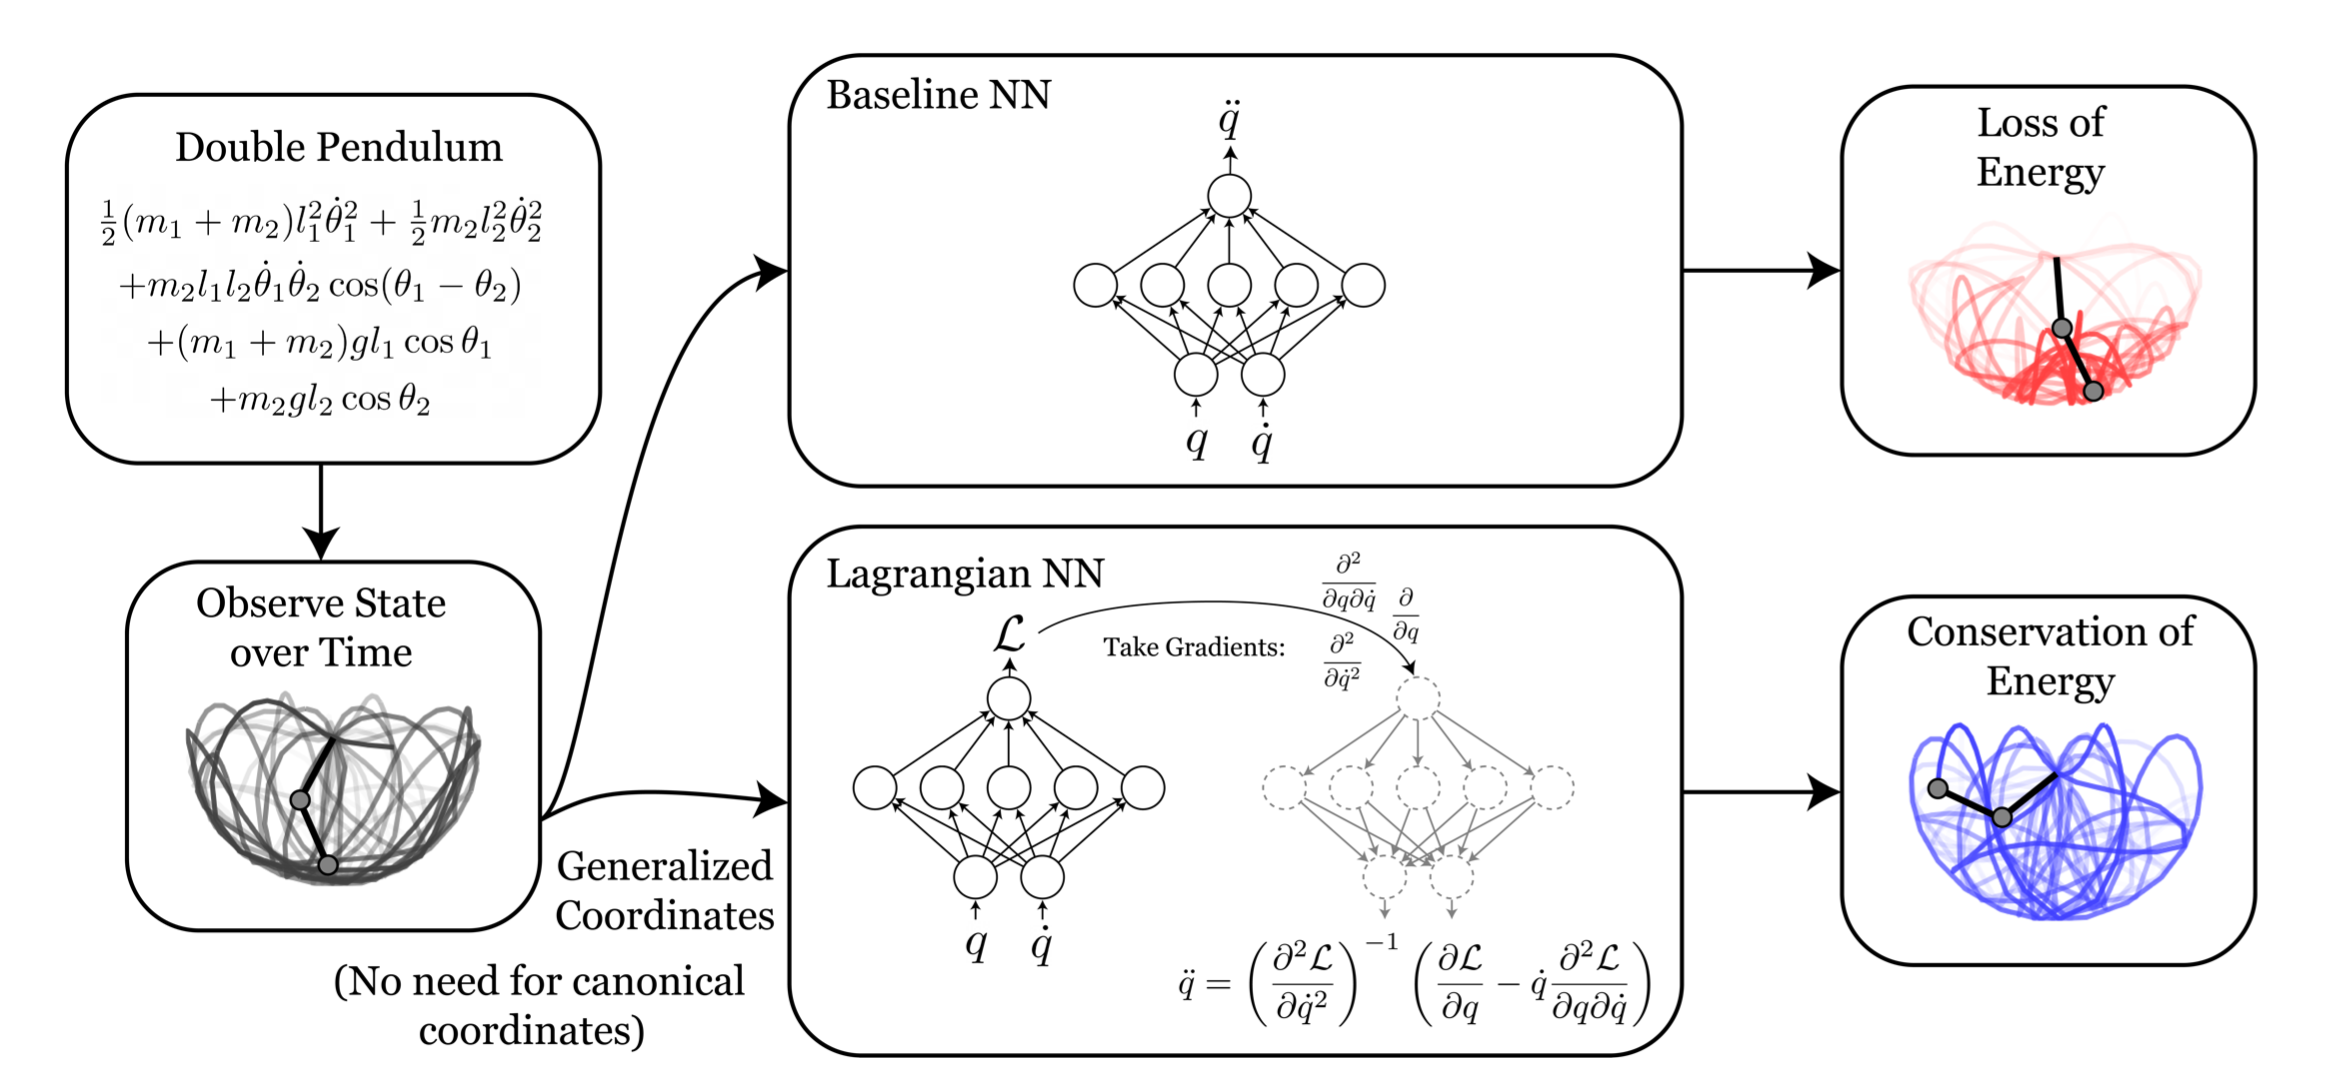
\includegraphics[width=0.99\textwidth]{lnn.png}
		\caption{Схема работы Lagrangian Neural Networks (LNN) моделирования динамики двойного маятника в сравнении с базовым решением (Baseline NN)}
	\end{figure}


	\textbf{Сравнение}
		\begin{figure}[h]
			\centering
			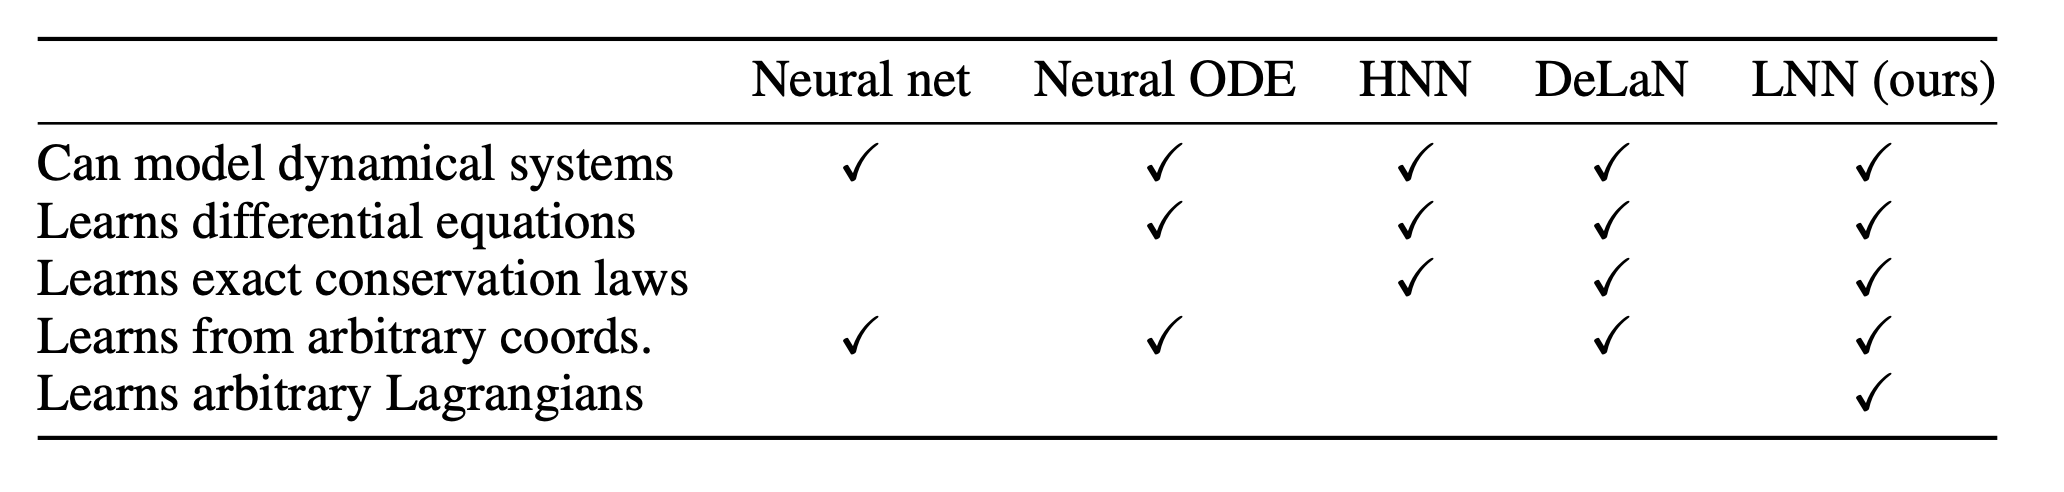
\includegraphics[width=1.05\textwidth]{comparison.png}
			\caption{Сравнение подходов моделирования физических систем нейронными сетями}
		\end{figure}
	

	
	\section{Вычислительный эксперимент}
	Целью вычислительного эксперимента является 
	В рамках вычислительного эксперимента написан программный комплекс для решения поставленных задач~\cite{source_code}.

	


	\section{Заключение}
	В работе рассмотрена задача 
	
	\bibliographystyle{unsrt}
	%\begin{thebibliography}{99}
		
	
	%	\bibitem{source_code}
%		\textit{Severilov}. Project source code is available at:~\url{https://github.com/severilov/BCI-thesis}, 2021.
	%\end{thebibliography}
	
\end{document}

